\mychapter{Potential Strength}{Potential  Strength}
Another parameter in our simulation which has a large influence on the behaviour of the system is the strength of the ellipsoidal potential. We varied this from $c_e =0$ to $c_e=30s^6$. The strength of the potential has two direct influences: A denser packing is penalized and  there is no hard threshold for the collision detection. The latter makes it easier for rods to escape from interlocking and thus facilitating the ordering process. The former slows down the sedimentation because the uppermost rod in  a stack of rods is pushed to the top by the rods below it. For a rod in the center of such a stack however, the potential does not prevent a dense packing since they are pushed both from above and below.   
\begin{figure}
  \begin{minipage}[t]{0.75\textwidth}
     \hspace{-0.1\textwidth}
     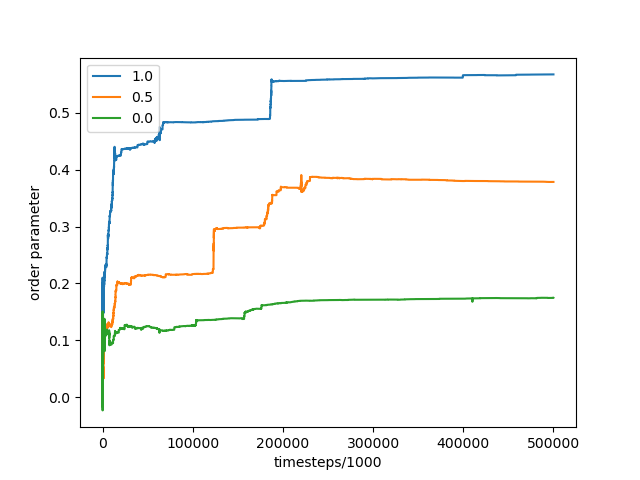
\includegraphics[width=1.2\textwidth]{data/pot_comb_order_parameter_three.png}
  \end{minipage}
  \hfill
  \begin{minipage}[b]{0.2\textwidth}
  {\setcapindent{0pt} \caption{Comparison of different potential strengths. We see that with stronger potentials, the particles seem to order more quickly. The materials used are iron and water.}}
  \vspace{25 pt}
\end{minipage}
\label{fig:pot_comp}
\end{figure}

